\documentclass[12pt]{article} 
\usepackage[francais]{babel}
\usepackage[T1]{fontenc}
\usepackage[utf8]{inputenc}
\usepackage{eurosym}
\usepackage{array}
\usepackage{graphicx}
\usepackage{fancyhdr}
\usepackage{verbatim}
\usepackage{enumerate}

\pagestyle{fancy}
\fancyhf{}
\rhead{Issidi}
\lhead{Rapport final}
\lfoot{Epita -- promotion 2020} //Insérer logo épita dans le lfoot //%
\includegraphics{epita.jpg}
\rfoot{Page \thepage}


\title{Rapport final\\
		Issidi\\
		Debil.OS();}
\author{Jérémy \bsc{Beuvry}\\
		Julien \bsc{Boulicaut}\\
		Clément \bsc{Finck}\\
		Sébastien \bsc{Fleury}\\
		\\
		Epita -- Promo 2020}

\begin{document}
\maketitle

\begin{figure}[!t]
\centering
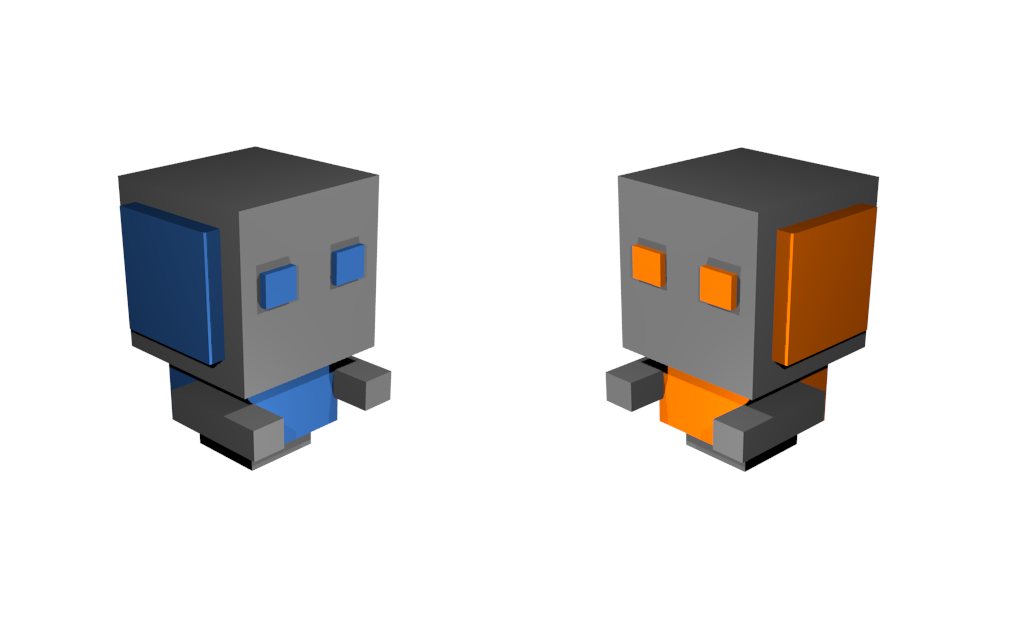
\includegraphics[scale=0.4]{front_page.png}
\caption{Des robots, personnages principaux}
\end{figure}

\newpage
\tableofcontents
\newpage
\listoffigures
\newpage

\section{Introduction}
Dans le cadre de notre première année préparatoire au sein d'Epita, 
il nous a été demandé de réaliser un projet informatique dont sujet
était libre.

/*
**Plus de blabla sur : "comprendre la position du projet au sein 
** de notre cursus"
*/

Ainsi, notre groupe, les ''Debil.OS();'' est fier de vous présenter son 
rapport final de son magnifique, que dis-je, génialissime projet :
Issidi.

Les auteurs de ce projet sont quatre compères de première année animés
d'une motivation à toute épreuve.

Ce projet prend la forme d'un jeu de tir à la troisième personne dans
un univers post apocalyptique. Les différentes mécaniques de jeu et
l'univers seront bien entendu détaillés dans la section adaptée.

La réalisation de ce projet Issidi nous a permit de nous confronter à
ce quii sera très probablement la réalité de notre futur métier
d'ingénieur : le travail en groupe. En effet, même si nous avons déjà eu
l'occasion de travailler en groupe au lycée ou pendant le premier semestre
, l'ampleur de ce projet nous montre l'efficacité, dans la répartition
des tâches comme dans la résolution des conflits, qui sera attendu
de nous lors de notre futur métier.

\section{Présentation}
\subsection{Présentation du projet}
\subsubsection{Scénario}
Dans un monde ravagé par la guerre tous les hommes sont mort ou
enterrés, mais pas nécessairement dans cet ordre. En effet, les
radiations résultant du grand bombardement de la troisième guerre
mondiale ont rendu la surface de la Terre létale pour l'humanité
telle que nous la connaissons. Les rares survivants sont contraints
de se terrer dans des bunkers antiatomiques pour pouvoir
espérer qu'il y ait un jour lointain un retour possible à la
surface. En attendant, seul des drônes peuvent se risquer au dehorts
pour récupérer des matériaux quand il en reste. Très vite, les
ressources se font rares et des luttes éclattent peu à peu. Incarnez
un pilote de drones de combat en récupérant un maximum de matériaux
nécessaires à la survie des camarades de votre abri et en déjouant
les assauts des autres pillards assoiffés de métal. Vous représenterez
l'ultime rempart entre la vie et la mort pour vos frères, alors,
laisserez-vous l'humanité sombrer sans agir ?

\subsubsection{Mécanique de jeu}
Issidi est un jeu de tir à la troisième personne (aussi appelé
\emph{Third Person Shooter}), qui sera créé avec le moteur de jeu
Unity3d, édition personnelle. A la différence des shooters
traditionels, plutôt horizontaux (souvent ramenés à un simple et
large plan horizontal avec des obstacles), Issidi a pour but
d’exploiter réellement les trois dimensions en permettant au
joueur de marcher sur les murs, mais aussi sur le plafond rendant
le jeu beaucoup plus dynamique! Ainsi, les possibilités de
déplacements du joueur seront démultipliées pour proposer une
expérience unique. En plus des déplacements classiques vous
pourrez également esquiver à l’aide de petit saut rapide vers
l’avant ou encore utiliser des doubles sauts qui permettront
aussi d’atteindre certaines zones qui auraient été inaccessibles
sinon. Attention toutefois à ne pas oublier où se trouve le sol
car un saut depuis un mur ou le plafond vous précipitera à terre
et même si votre etes solide, selon la hauteur, une telle chute
vous sera sans doute fatal. De plus, dans le mode solo, la caméra
à la troisième personne vous permettra de mieux appréhender votre
environement ce qui vous permettra après réflexion de choisir votre
chemin que ce soit : au plafond, sur les murs ou tout simplement
au sol. Et ne croyez pas que ce sera une tâche aisée, votre
environement étant en ruine et partiellement truffés d’appareils
en tous genres présent uniquement pour vous réduire en pièces
détachées, toutes les routes ne seront pas empruntables soit
parcequ’elles seront bouchées, soit à cause des diverses tourelles
et autres joyeuses défenses automatiques qui vous bloqueront
définitivement le passage, vous forçant à rebrousser chemin, vous
forçant à rebrousser chemin dans l’espoir d’en trouver un autre
dans ces dédales de débris. Plusieurs armes seront disponibles
pour varier le gameplay et permettre à tous les types de joueurs
de prendre un maximum de plaisir. Le mode multijoueurs mettra en
scène les batailles sanglantes entre pillards de ressources dont
un seul sortira vainqueur, ou pas!



\subsection{Présentation des membres de l'équipe}
\subsubsection{Julien \bsc{Boulicaut}, chef de projet}
En tant que chef de projet, je tiens tout d'abord à remercier Epita qui nous
donne l'opportunité de réaliser un de nos rêves d'enfant : créer un jeu vidéo.
Passionné d'informatique depuis tout petit, j'ai commencé les tutoriels de
programmation en fin de 3ème au collège. Puis durant le lycée, je me suis contenté
de quelques programmes sur ma calculatrice ainsi que de la création de sites web.
Habitué à remplir le rôle de chef d'équipe dans la plupart des groupes auquel
j'ai participé, j'ai été choisi à l'unanimité pour assurer cette fois encore
cette fonction dans notre petite équipe. Je m'engage à maintenir la communication
entre les membres du groupe, notamment en instaurant une réunion hebdomadaire afin
d'éviter, je l'espère, d'avoir à faire des rush trop importants. Cette réunion aura
aussi pour but de faire le point au sein du groupe concernant les tâches précises 
de chacun afin d'éviter de perdre du temps en ayant des redondances dans les travaux
réalisés.

Je suis très enthousiaste concernant ce projet, et cela pour plusieurs raisons.
La première étant que j'ai la chance d'être avec trois autres personnes dont je sais
qu'elles s'investiront à 100\% dans le projet. Je suis aussi très satisfait du principe
d'Issidi que nous avons construit ensemble pendant nos pauses repas. Pour finir, je
suis très excité à la perspective d'en apprendre plus, que ce soit en C\# ou en HTML,
CSS ou encore PHP et de pouvoir enfin jouer à ce jeu auquel nous réfléchissons depuis
déjà quelques mois.

\subsubsection{Jérémy \bsc{Beuvry}}
Ayant commencé la programmation depuis déjà 4 ans, je mettrai à profit les compétences
apprises lors de projets personnels, nombreux mais pas finis. En effet, ce projet issu
d'une longue réflexion au sein de notre groupe et avec un grand potentiel me permettra
dans ce projet de grande envergure d'utiliser intelligemment ce que j'ai appris précédemment,
dans un groupe avec une excellente entente en son sein. De plus, ce projet m'apprendra
le travail en équipe, qui est une compétence fondamentale dans le monde d'aujourd'hui,
ainsi que l'apprentissage d'un nouveau langage qu'est le C\#, qui m'était totalement
inconnu avant mon entrée à Epita. Ainsi, c'est avec un énorme sourire aux lèvres que
je m'apprête à commencer ce projet. 

\subsubsection{Clément \bsc{Finck}}
J'ai très peu codé dans ma vie mais j'ai toujours eu envie de participer à ce genre de
projet et Epita me donne l'opportunité de pouvoir participer enfin à ceci. Créer un jeu
vidéo a toujours fait partie de mes rêves même si je n'ai jamais réussi à passer le cap
tout seul. Je saisis cette occasion pour pouvoir montrer ce que je peux faire en me
donnant à 200\%. De plus je suis très confiant par rapport à mon groupe car je sais
que tous autant qu'ils sont, ils seront se donner à fond afin que celui-ci soit le
meilleur possible. J'ai très envie de pouvoir aider mon équipe autant que possible et
je pense vraiment que ce projet sera une réussite. Je suis très content de l'idée
centrale de notre projet car je la trouve très originale et efficace car je ne connais
aucun jeu basé sur un tel gameplay. De plus, je pense que notre équipe sera un très 
bon moyen pour moi d'améliorer mes connaissances en codage et cela me ravit. 

\subsubsection{Sébastien \bsc{Fleury}}
Pendant longtemps j'ai voulu automatiser plusieurs tâches sur mon ordinateur, ce qui
m'amena à apprendre en 3\ieme la programmation. C'est donc depuis 4 ans que je travaille
régulièrement sur le framework .NET et plus récemment Java. J'ai eu la chance aussi de
pouvoir travailler sur d'autres types de compilateur avec une API bien moins complète
et intuitive. Ce projet m'enseignera une meilleure pratique du travail d'équipe, plus
importante que celle que j'ai actuellement et l'utilisation d'un autre moteur graphique,
ayant utilisé XNA, nativement celui du .NET. J'ai donc comme tout notre groupe beaucoup
à apprendre en travaillant sur ce projet. J'ai de plus la chance de travailler avec des
camarades non seulement très impliqués dans le projet, mais aussi et surtout très sympathiques,
ouverts aux suggestions et capables de trouver des solutions aux problèmes.

\section{Découpage du projet}
\subsubsection{Physique}
Cette section sera dédiée à la gestion des interactions des différents élements avec
la gravité. Ainsi que la gestion de tous les types de collisions : joueur/terrain,
projectile/joueur, projectile/terrain (pour à terme, permettre d’avoir un environnement
partiellement destructible).
Parmi les interactions on notera en particulier la possibilité de marcher sur les murs 
et le plafond, via un changement de gravité, ce qui constituera l’une des pricipales
mécaniques du jeu.

\subsection{Mode un joueur}
Le mode solo consistera à parcourir les ruines de vieilles usines abandonnées à la recherche
de tout ce qui pourrait être utile à votre survie. Il faudra donc essayer de ne pas se faire
tuer par les défenses automatiques encore actives et de se frayer un chemin parmi les décombres.

\subsection{Multijoueur}
Le multijoueur est un point important de ce projet.
En effet, même s’il disposera d’un mode solo, l’intérêt principal d’ Issidi résidera dans les
affrontements épiques entre joueurs. Le réseau ne permettra donc pas seulement d’allonger
la durée de vie du jeu mais aussi d’enrichir l’expérience de celi-ci. Il sera capable
de regrouper jusqu’à ”42” joueurs dans des modes de jeux divers et variés (deathmatch, capture de drapeau...).

\subsection{Intelligence artificielle}
Nous aurons besoin de deux types d’Intelligence Artificielle (IA) dans Issidi.
Premièrement, il faudra un système de visée pour les tourelles qui défendront
les usines désaffectées. Deuxièmement, la création de pathfiding pour les systèmes
de défense mobile sera aussi nécessaire (de gentilles araignée mécaniques dont leurs
seul but sera de se faire sauter à votre proximité).

\subsection{Particule}
Afin d’améliorer la beauté de ce projet, l’ajout de particules est indispensable!
On pourra par exemple faire apparaitre la trainée des differents projectiles, afin de
montrer leurs trajectoires. Ou encore de dynamiser l’action et d’égailler les décors.

\subsection{Personnage}
Comment jouer sans personnage ? Cela semble en effet plutôt complexe, pour cela
nous donnerons vie à de mignons petits robots qui pourront répandre la democratie
américaine. Les joueurs auront non seulement la possibilité de se déplacer sur le sol,
mais aussi sur les murs ou le plafond du terrain. Une bonne gestion des déplacements
et de la caméra est donc indispensable, dans un monde où l’on peut se retrouver face
à un ennemi la tête à l’envers!

\subsection{Arme}
Un robot sans défense n’a aucun interêt s’il ne possède rien lui permetttant
d’occire ses ennemis, il doit donc disposer d’un arsenal suffisant. Il sera donc
nécéssaire de créer plusieurs armes afin d’ajouter une profondeur au gameplay.

\subsection{Son}
Que serait un jeu sans son? Le but ici sera de créer une bande son simple mais orignale.

\subsection{Création des modèles}
Tout jeu digne de ce nom doit aussi avoir des graphismes à la hauteur! C’est pourquoi
cette partie consistera à la réalisation des modèles nécessaires afin de réaliser
notre projet, et lui donner une ambiance qui le différenciera des autres jeux post
apocalyptiques. Seront inclus la création des personnages ainsi que les environements.

\subsection{Interface}
Afin de rendre le jeu plus convivial, celui-ci doit posséder une interface composée
de plusieurs menus. Celle-ci permettra notamment de naviguer dans les options du jeu,
de lancer une partie en mode solo, ainsi que de choisir les paramètres des parties
du mode multijoueur.

\subsection{Site web}
Le site web nous permettra de montrer l’avancement de notre projet.
Il contiendra une description du projet, des images de celui-ci, ainsi que des
liens permettant d’avoir un accès rapide aux sources du projet.

\section{Répartition des taches}
\begin{tabular}{|c|c|c|c|c|}
\hline
			&	Jérémy		&	Julien		&	Clément		&	Sébastien	\\ \hline
Site Web	&				& $\bigotimes$	& 				& $\bigcirc$	\\ \hline
Physique	&				&				& $\bigcirc$	& $\bigotimes$	\\ \hline
Multijoueur	& $\bigotimes$	& $\bigcirc$	&				& 				\\ \hline
Animation	&				& $\bigotimes$	& $\bigcirc$	&				\\ \hline
IA			& 				& $\bigotimes$	& $\bigotimes$	&				\\ \hline
Particules	& $\bigcirc$	& 				&				& $\bigotimes$	\\ \hline
Personnage	& $\bigotimes$	&				& 				& $\bigcirc$	\\ \hline
Arme		& $\bigcirc$	&				&				& $\bigotimes$	\\ \hline
Son			&				& $\bigcirc$	& $\bigotimes$	&				\\ \hline
Modèles		& $\bigotimes$	&				& $\bigotimes$	&				\\ \hline
Interfaces	& 				& $\bigcirc$	& $\bigotimes$	&				\\ \hline
\end{tabular}

Légende:\\
$\bigotimes$ : s'occupe de\\
$\bigcirc$ : aide

\section{Avancement du projet}//Renommer cette catégorie si plus d'idée
On NE parle PAS de code, mais du général, ce qu'on à fait.
Description de ce qu'il y a dans le projet quoi.


\section{Bilan du projet}
Bilan sur nous et notre groupe.
Pas le même bilan au sein du groupe.
On ne s'agresse pas (dommage...)

\section{Conclusion}

\section{Bibliographie}
LOL... (en plus faut la commenter)

- docs.unity.com
- stackoverflow.com